\subsection{Hochspannung der Photomultiplier}
Ein exaktes Einstellen der Photomulitplier ist  essenziell f�r eine gute Messung. Die Spannungen von PM2 und PM4 sollen dabei einen Wert von 2200 V nicht �berschreiten. Die Spannung von PM1 soll 2000V nicht �bersteigen. Der Arbeitspunkt von PM3 liegt im Bereich von 2700-3000 V, wobei ein Wert von 3000V nicht �berschritten werden soll. F�r die Bestimmung des optimalen Arbeitspunktes wird die Schwelle des Diskriminators auf einen m�glichst geringen Wert eingestellt. Es wird der Logarithmus der Z�hlrate in Abh�ngigkeit der Spannung untersucht und nach dem Punkt, an dem die Steigung abknickt gesucht, da sich der Photomulitplier dann am optimalen Arbeitspunkt befindet. Die Z�hlrate wird logarithmisch aufgetragen, wobei ein $^{60}Co$-Pr�parat verwendet wird, um die Z�hlrate zu erh�hen.
Die aufgenommenen Spannungskennlinien sind in Abbildung \ref{fig:hoch_1} bis \ref{fig:hoch_4} zu sehen.

%Auswertung der Spannungskennlinien, beschreibung der Plots
\begin{figure}[H]
	\centering
  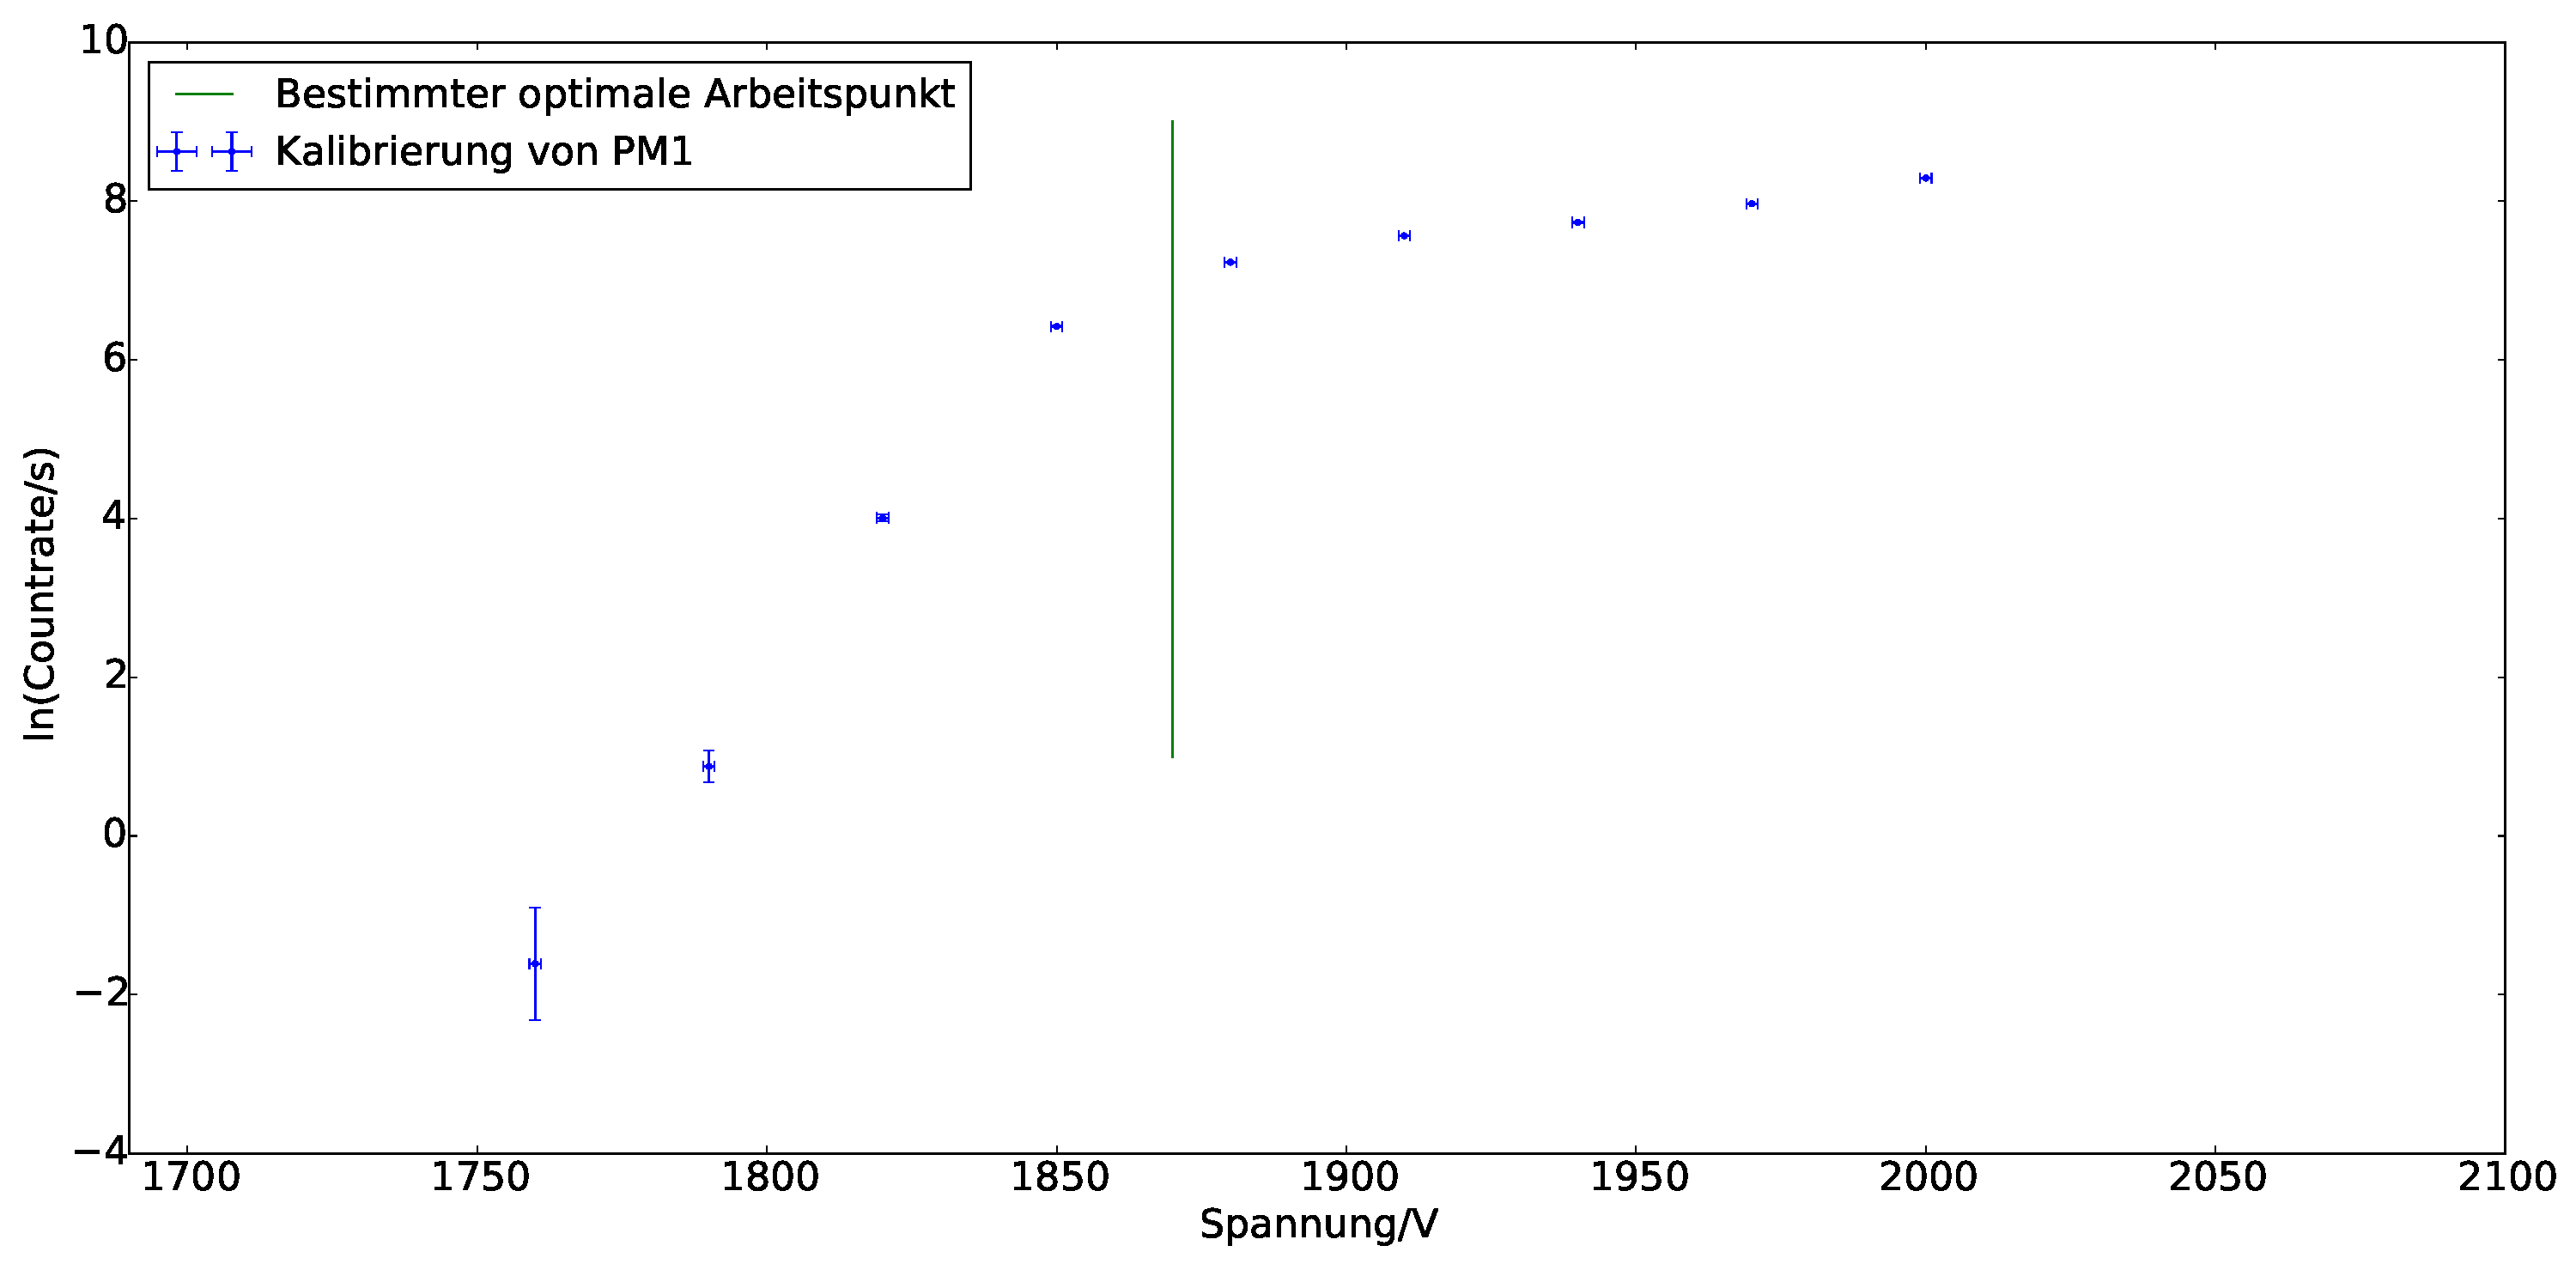
\includegraphics[scale=0.33]{pm_1_spannung.pdf}
	\caption{Messung der Z�hlrate in Abh�ngigkeit der Spannung f�r die ersten Photomulipier. Es wurde ein $^{60}Co$-Pr�parat verwendet, um die Z�hlrate zu erh�hen. Der Abknick wurde bei einer Spannung von 1870V bestimmt.}
	\label{fig:hoch_1}
\end{figure}

\begin{figure}[H]
	\centering
  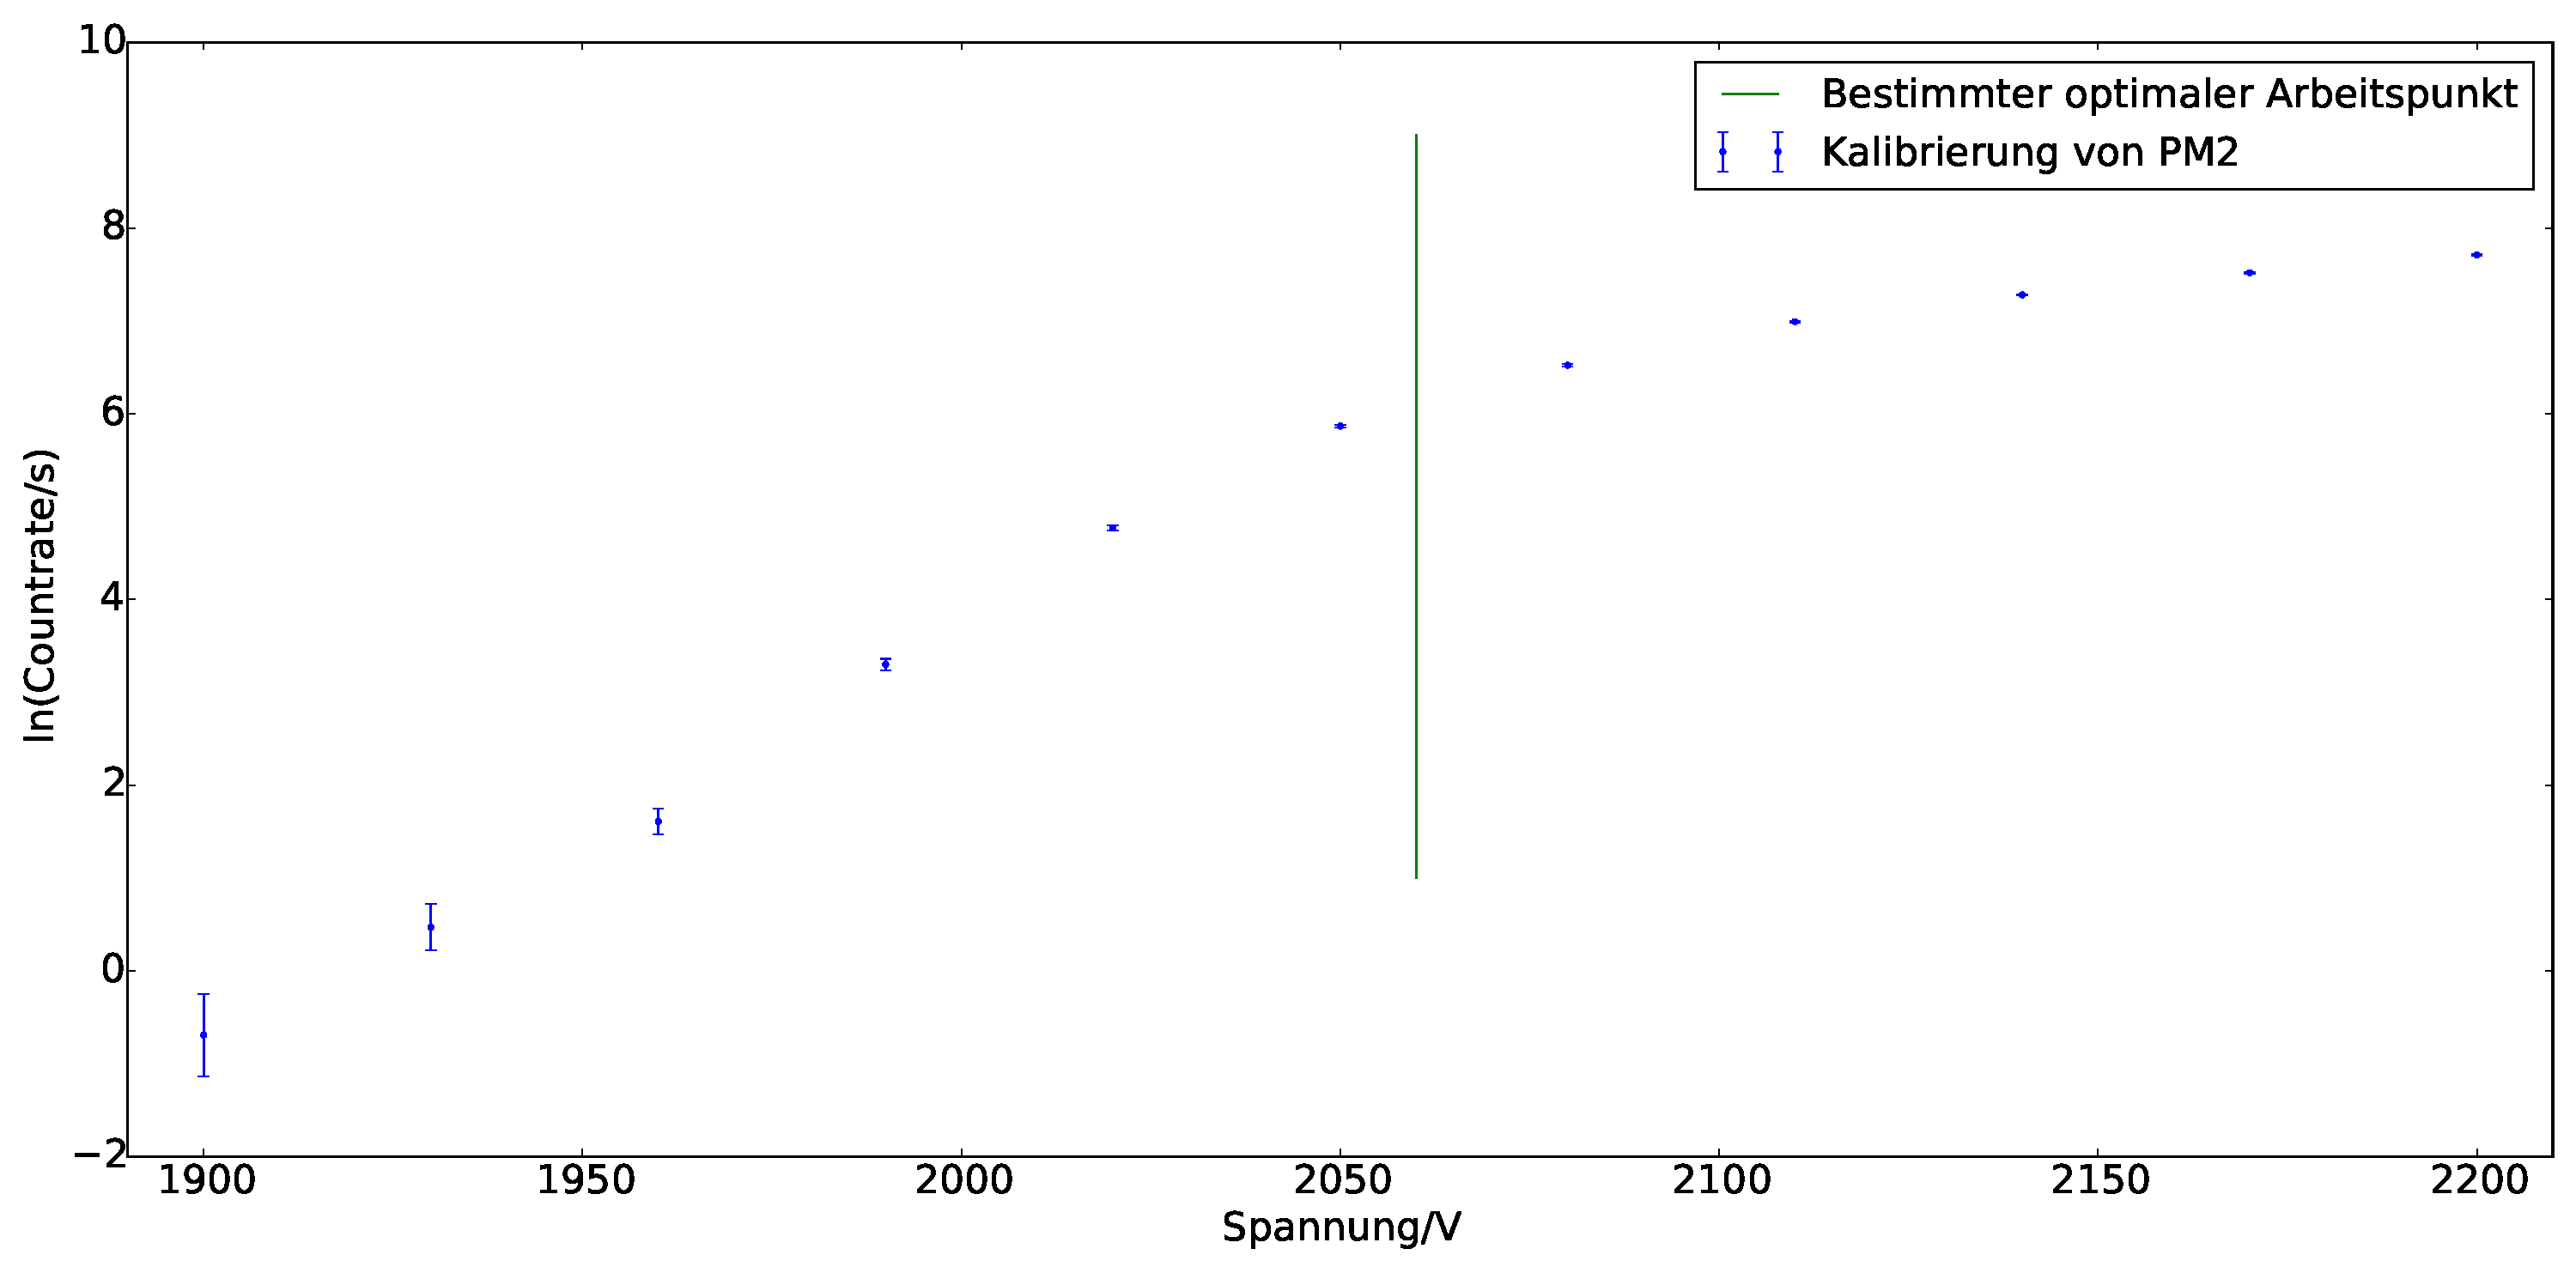
\includegraphics[scale=0.33]{pm_2_spannung.pdf}
	\caption{Messung der Z�hlrate in Abh�ngigkeit der Spannung f�r die zweiten Photomulipier. Es wurde ein $^{60}Co$-Pr�parat verwendet, um die Z�hlrate zu erh�hen. Der Abknick wurde bei einer Spannung von 2060V bestimmt.}
	\label{fig:hoch_2}
\end{figure}

\begin{figure}[H]
	\centering
  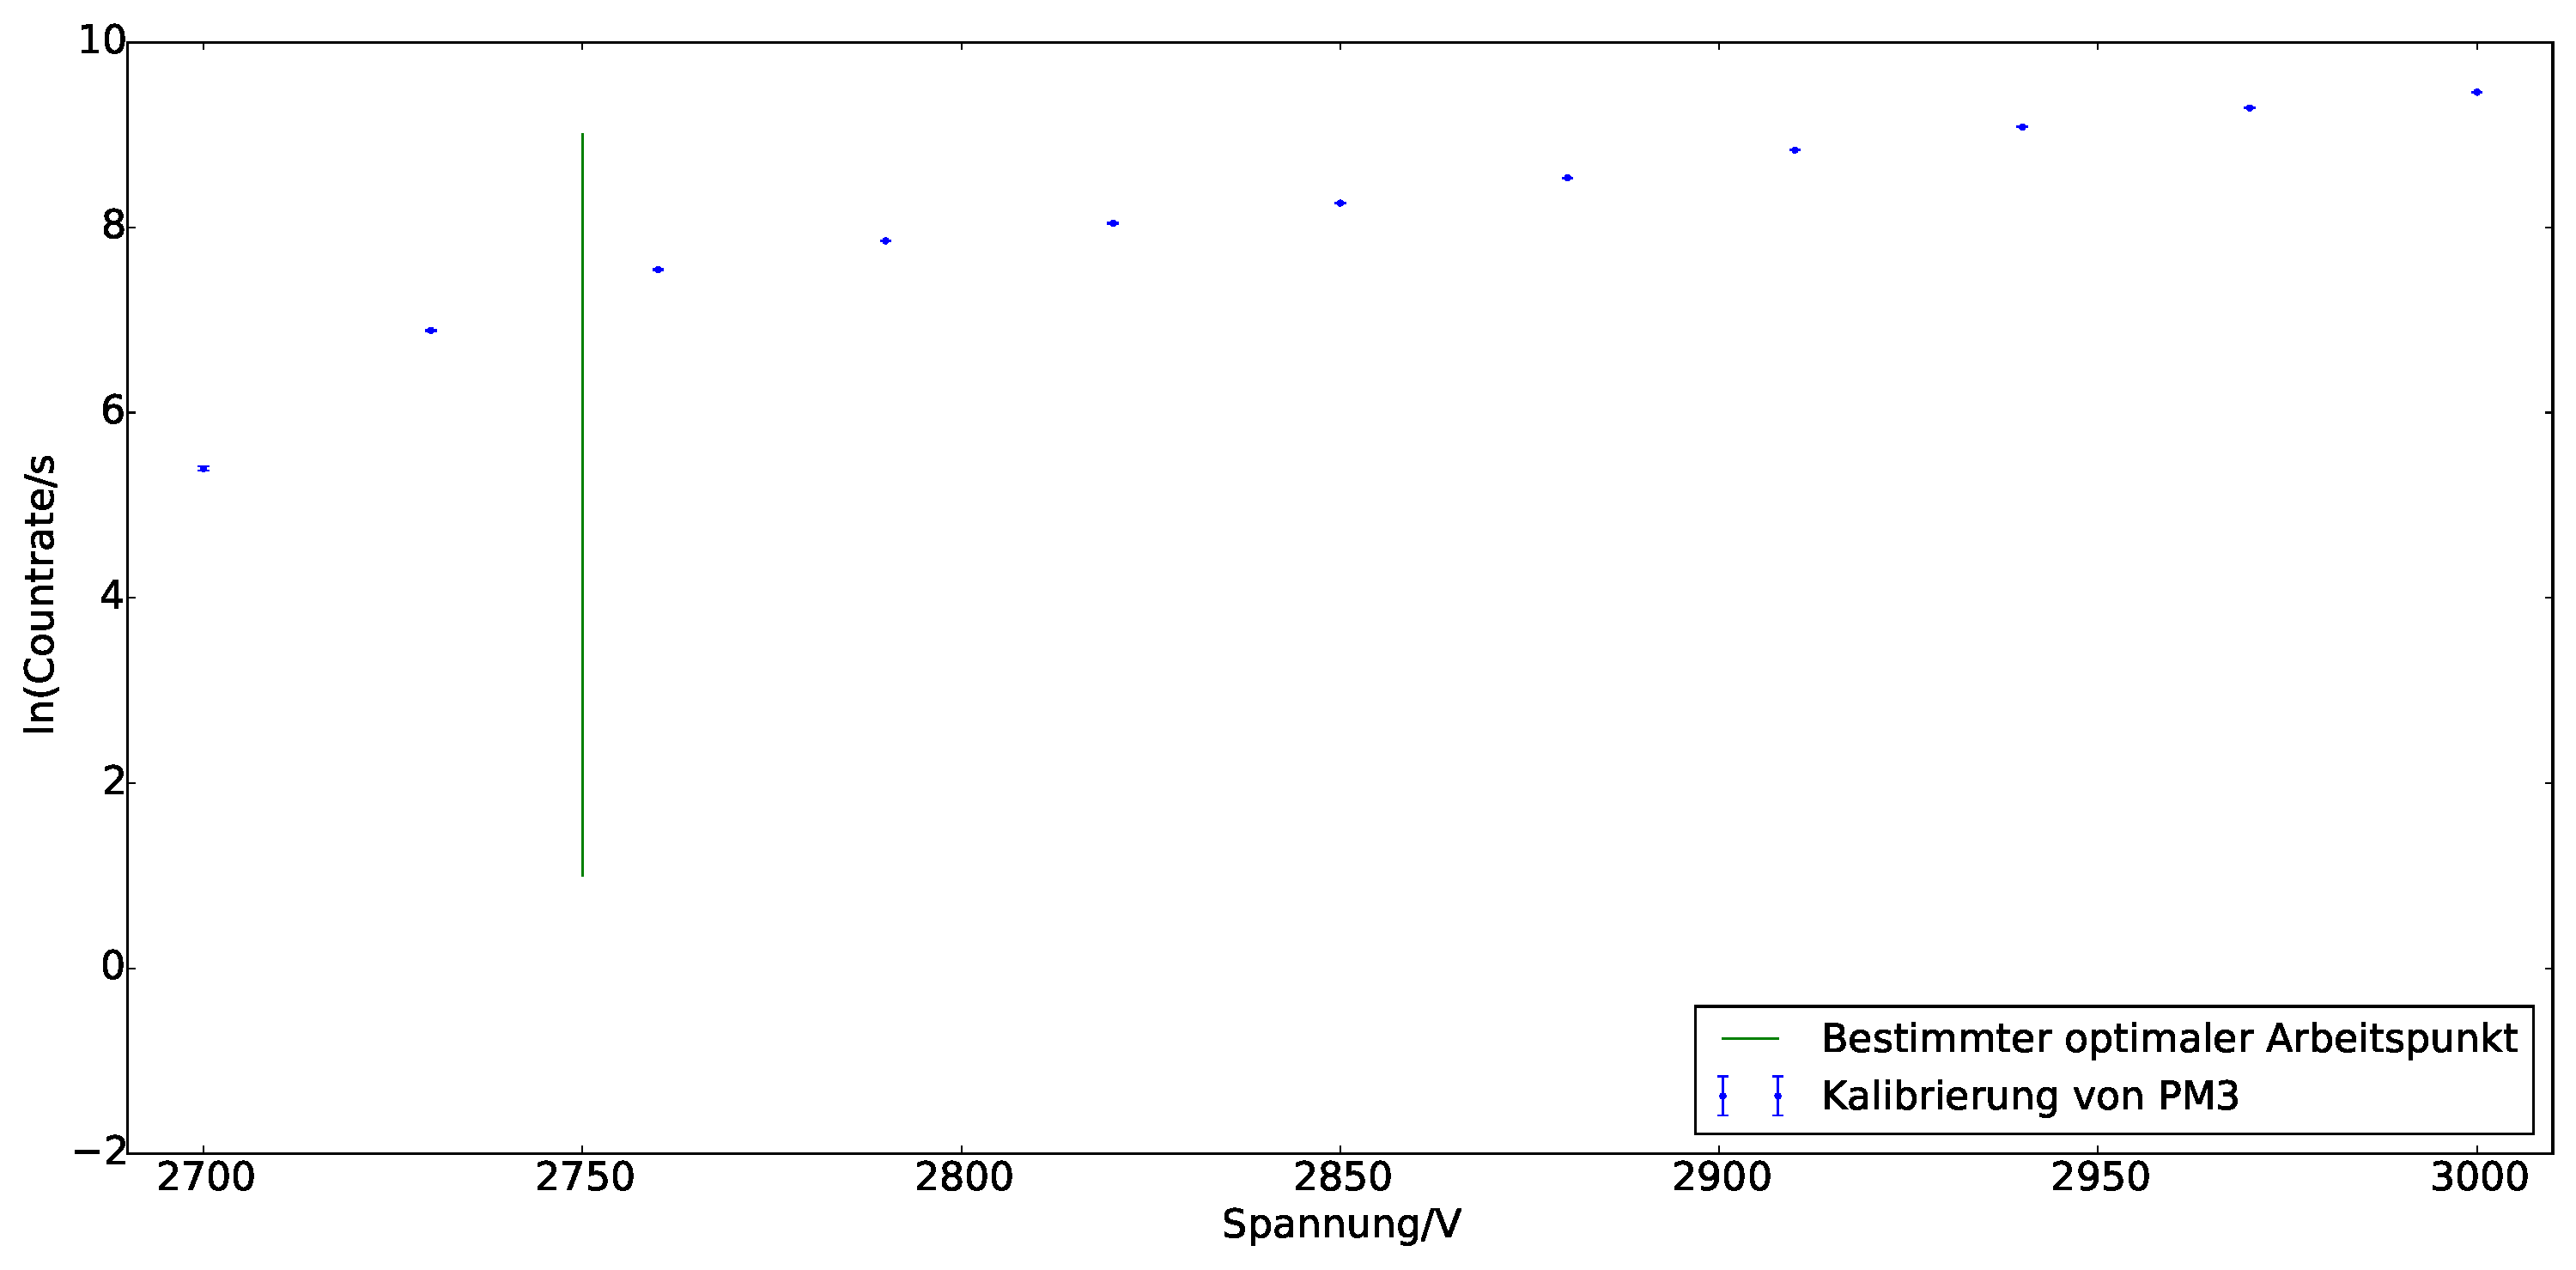
\includegraphics[scale=0.33]{pm_3_spannung.pdf}
	\caption{Messung der Z�hlrate in Abh�ngigkeit der Spannung f�r die dritten Photomulipier. Es wurde ein $^{60}Co$-Pr�parat verwendet, um die Z�hlrate zu erh�hen. Der Abknick wurde bei einer Spannung von 2750V bestimmt.}
	\label{fig:hoch_3}
\end{figure}

\begin{figure}[H]
	\centering
  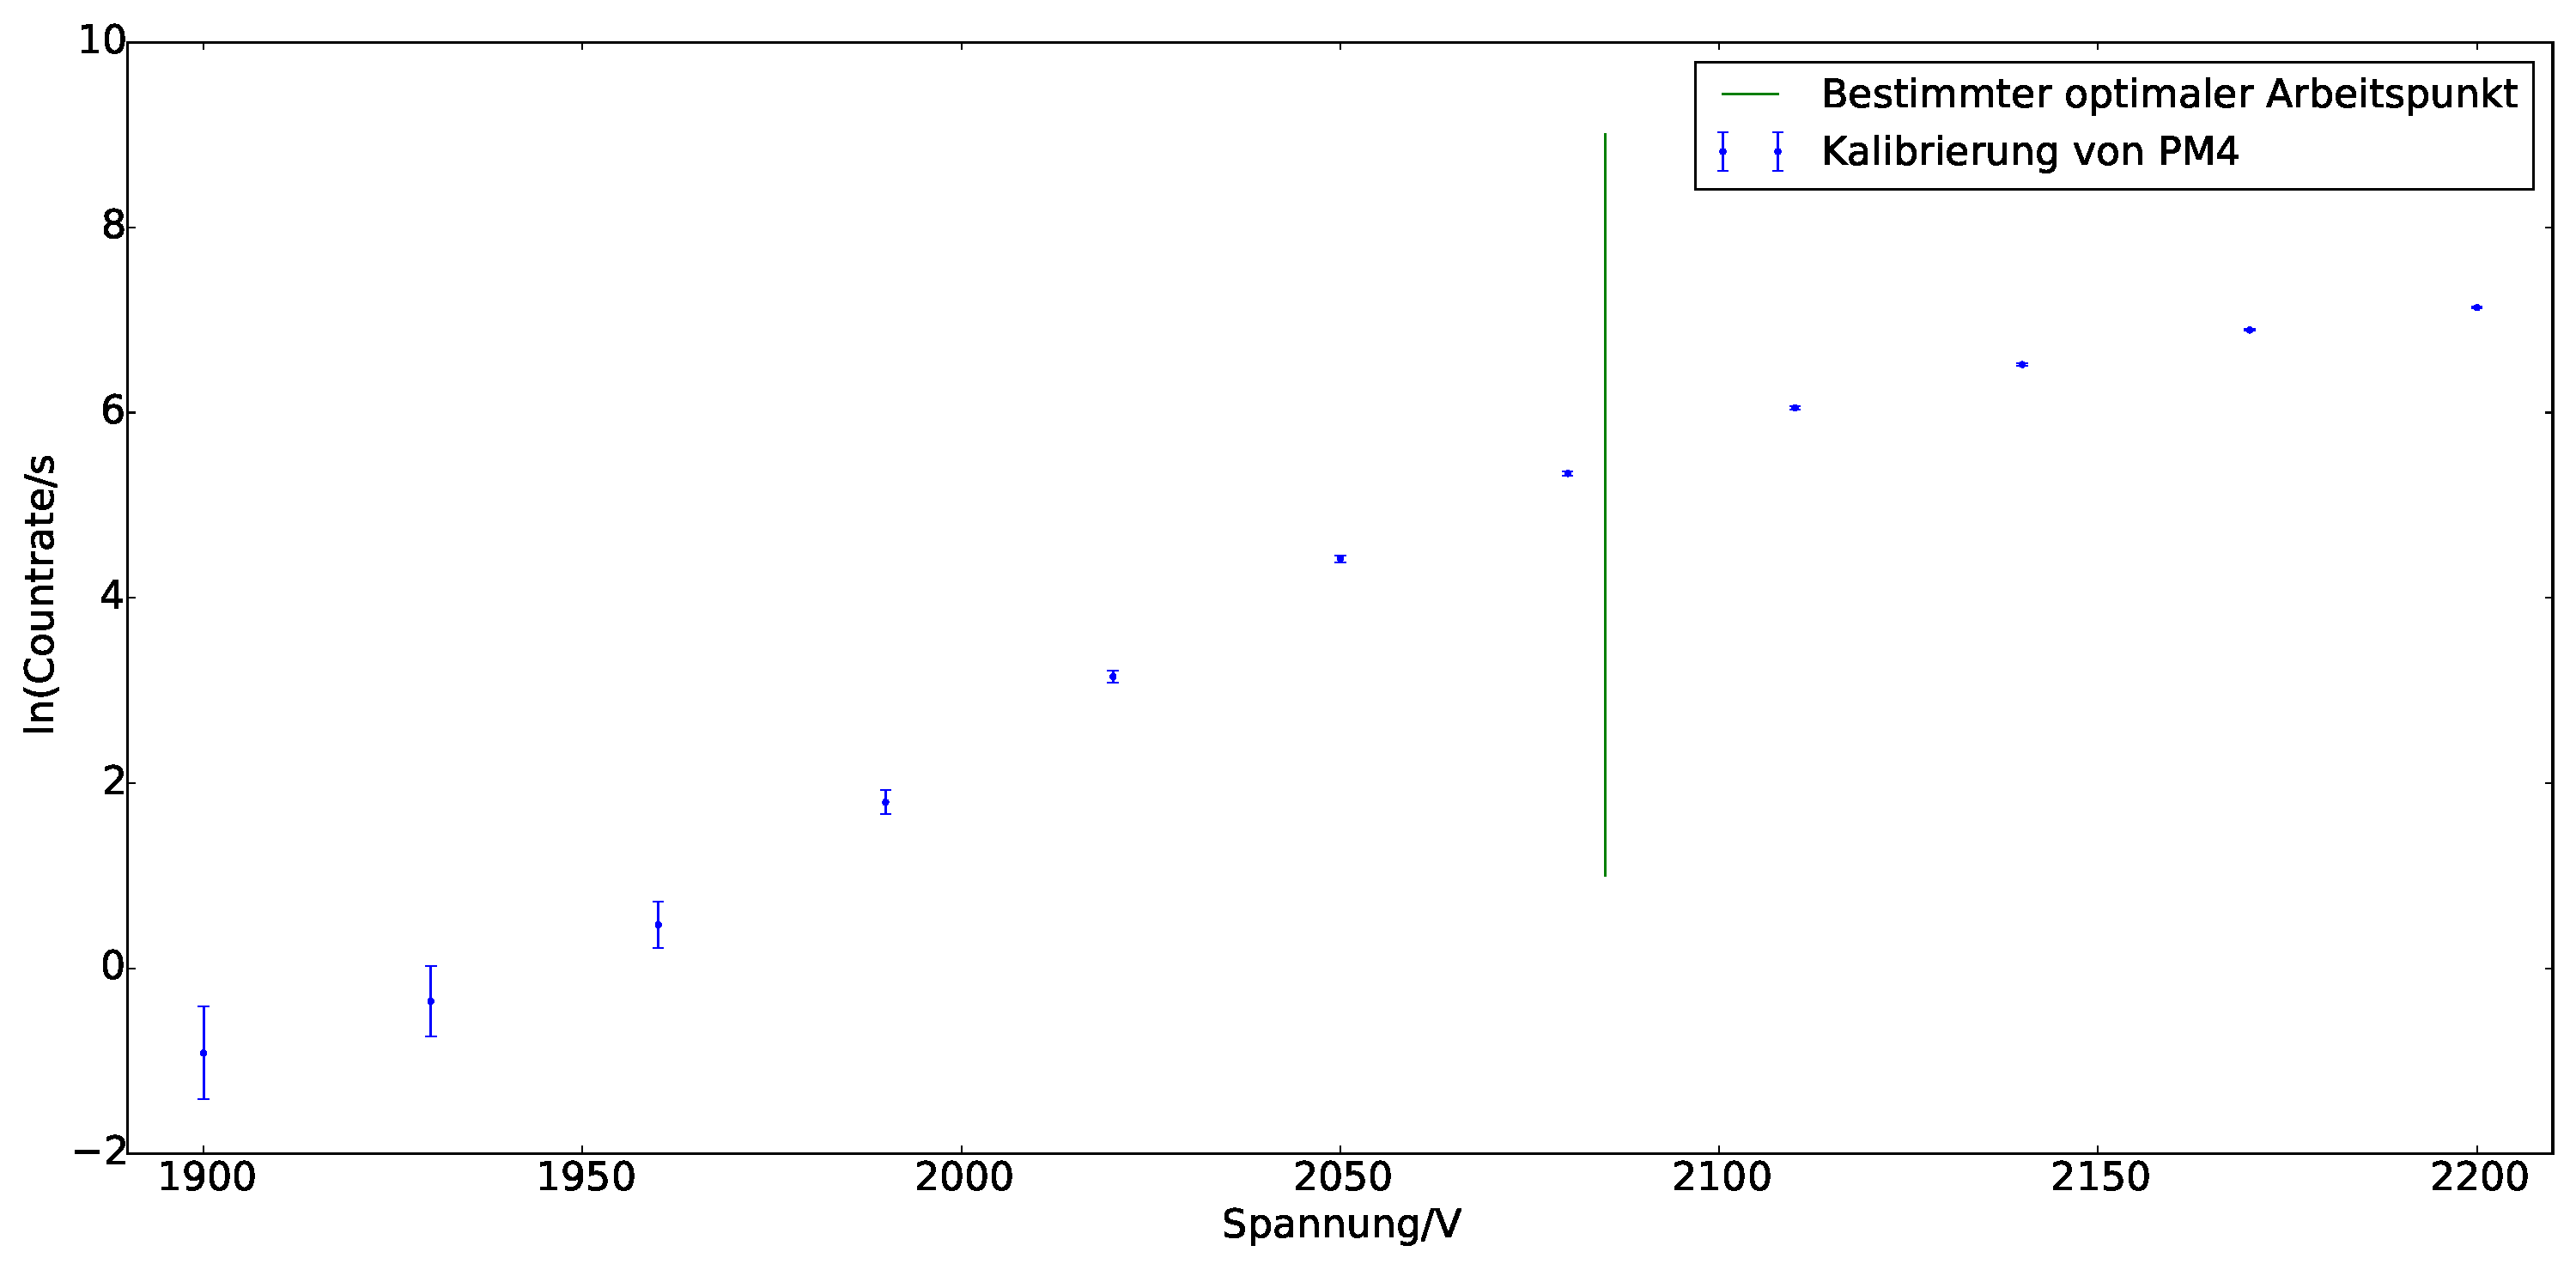
\includegraphics[scale=0.33]{pm_4_spannung.pdf}
	\caption{Messung der Z�hlrate in Abh�ngigkeit der Spannung f�r die vierten Photomulipier. Es wurde ein $^{60}Co$-Pr�parat verwendet, um die Z�hlrate zu erh�hen. Der Abknick wurde bei einer Spannung von 2085V bestimmt.}
	\label{fig:hoch_4}
\end{figure}

Die bestimmten Spannungen f�r die Photomulitplier sind in Tabelle \ref{tab:hochspannung} aufgetragen.

\begin{table}[H]
\centering
\caption{Verwendete Spannungen f�r die Photomuliplier}
\label{tab:hochspannung}
\begin{tabular}{|c|c|}
\hline Photomultiplier & Spannung[V] \\ \hline
\hline PM1 & 1870 \\ 
\hline PM2 & 2060 \\ 
\hline PM3 & 2750 \\ 
\hline PM4 & 2085 \\ 
\hline 
\end{tabular} 
\end{table}